%%%%%%%%%%%%%%%%%%%%%%%%%%%%%%%%%%%%%%%%%%%%%%%%%%%%%%%%%%%%%%%%%%%%%%%%%%%%%%%%
%% Capitulo
%%%%%%%%%%%%%%%%%%%%%%%%%%%%%%%%%%%%%%%%%%%%%%%%%%%%%%%%%%%%%%%%%%%%%%%%%%%%%%%%
\chapterimage{chapter_head_2.pdf} % Chapter heading image

\chapter{Estilos de dança no samba}

%%%%%%%%%%%%%%%%%%%%%%%%%%%%%%%%%%%%%%%%%%%%%%%%%%%%%%%%%%%%%%%%%%%%%%%%%%%%%%%%
%%%%%%%%%%%%%%%%%%%%%%%%%%%%%%%%%%%%%%%%%%%%%%%%%%%%%%%%%%%%%%%%%%%%%%%%%%%%%%%%
\section{Que estilos de dança posso usar no samba (música)?}
\label{subsec:estilosdedanca}
A resposta mais simples poderia ser que, uma pessoa ao ser livre e independente,
pode escolher expressar-se na dança, de forma natural, como esta saia de si mesmo.
Porem, entrando em assuntos mais técnicos, 
e de acordo com os padrões socialmente mais comuns de ser achados atualmente;
existe um grupo de modalidades de dança, que por suas caraterísticas, 
são consideradas que se enquadram muito bem na música de alguns subgêneros do samba.

Assim, nas seguintes seções, serão descritos alguns dos estilos de dança para a música do samba,  
que podemos achar nos salões e locais de dança no Brasil;
estes serão agrupados em estilos \textbf{dançados em pares}, e os que são \textbf{dançados de forma separada}. 


%%%%%%%%%%%%%%%%%%%%%%%%%%%%%%%%%%%%%%%%%%%%%%%%%%%%%%%%%%%%%%%%%%%%%%%%%%%%%%%%
\section{Estilos dançados em pares}
\label{subsec:estilosdedancapares}
Entre os estilos que se dançam a dois, existentes na atualidade, temos \cite[pp. 134]{perna2002samba}:

%%%%%%%%%%%%%%%%%%%%%%%%%%%%%%%%%%%%%%%%%%%%%%%%%%%%%%%%%%%%%%%%%%%%%%%%%%%%%%%%
\subsection{Samba de gafieira (dança)} 
\index{Dança!Samba de gafieira}
É uma dança a dois, que pode ser executada na maioria dos subgêneros do samba (música),
tendo exceções em: samba-enredo, samba reggae (música), samba rock (música), 
marcha, marcha-rancho e maxixe (música) \cite[pp. 134]{perna2002samba}.
No seus origens este tipo de dança era chamado de samba-batucada  \cite[pp. 134]{perna2002samba}. 
Para mais detalhes sobre o samba de gafieira, ver Seção \ref{cap:sambagafieira}.

%%%%%%%%%%%%%%%%%%%%%%%%%%%%%%%%%%%%%%%%%%%%%%%%%%%%%%%%%%%%%%%%%%%%%%%%%%%%%%%%
\subsection{Samba liso} 
\index{Dança!Samba liso}
%\index{Dança!Samba caminhado}
Atualmente se dança similarmente ao samba de gafieira, 
porem com um estilo mais elegante, sem ginga né passos de efeito, e dizer é uma dança mais ``lisa'';
se dança bem em : samba-canção, bossa nova e choro \cite[pp. 134]{perna2002samba}.~\\

\PRLsep{Referencias ao samba liso (1917-1933):} 

Podemos achar uma referencia interessante ao uso do termo \textbf{samba} e \textbf{liso}  no livro 
``Feitiço decente: Transformações do samba no Rio de Janeiro (1917-1933)'' (2001),
onde se pode intuir a procedência deste nome ou denominação, 
quando se faz referencia a um comentário de João da Baiana sobre o samba-de-umbigada e o samba de roda \cite[pp. 109]{sandroni2001feitico}: 
\begin{citando}
Nós tirávamos um verso e o pessoal sambava, um de cada vez ... 
Um saía para tirar o outro.
Se fosse a ``liso'' era só umbigada, mas se fosse para pegar ``duro'' já era capoiragem. 
\end{citando}
Pelo que no livro se comenta, que para o dançarino solista  escolher a seu sucessor podiam
existir duas modalidades, dependendo do tipo de roda, em ``samba liso'' (com umbigada) ou em ``samba duro'' 
(ou batucada\footnote{No qual a umbigada é substituída por uma pernada \cite[pp. 109]{sandroni2001feitico},
para mais detalhes ir a página \pageref{ref:batuquedanca}.}) \cite[pp. 109]{sandroni2001feitico}.
Esta referencia 
é particularmente interessante, pois como veremos na Seção \ref{cap:sambagafieira},
nos primórdios do samba nas gafieiras, existiam 3 modalidades em que esta era dançada: samba-canção (dança),
\textbf{samba-batucada} (dança)\footnote{Que 
é o nome com que era conhecido originalmente a atual samba de gafieira \cite[pp. 143]{perna2002samba}.} 
e \textbf{samba-liso} \cite[pp. 143]{perna2002samba};
estas duas últimas, não são as mesmas danças dos samba-de-umbigada, 
e sim novas formas de dançar o samba num ambiente mais civilizado como o salão de dança;
porem, estes nomes conservavam a mesma nomenclatura, na descrição 
da relativa relação à tosquedade dos movimentos, entre uma dança mais suave ou lisa, 
e outra dura ou batucada.~\\

%%%%%%%%%%%%%%%%%%%%%%%%%%%%%%%
\PRLsep{Referencias ao samba liso (1950-1953)}

Na ``Hemeroteca Digital Brasileira'' da Fundação Biblioteca Nacional,
não tem-se achado referencias\footnote{ Foram achadas,
2, 5, 3, 1 e 1 referencias brutas para as décadas de 1930, 1940, 1960, 1970 e 1980 respetivamente;
porem, estas não eram relativas ao samba liso de salão ou eram falsos acertos.} 
à frase ``\textbf{samba liso}'', nas décadas de 1930, 1940, 1960, 1970 e 1980;
as referencias achadas correspondem à década de 1950\footnote{Especificamente entre os anos 1950 e 1953.}  
com uma total de 327 referencias;
de todas estas, 326 correspondem à forte campanha 
de marketing do livro
``Como aprender a dançar'' , 
de Gino Forniciari. 
Por exemplo, podemos achar a primeira referencia em ``O Jornal'' (RJ),
do dia 17 de setembro de 1950, onde se pode ler \cite[3ra seção pp. 9]{jornalanunciodanca1}:
\begin{citando}
\begin{center}
Como aprender a dançar\\
4a edição ampliada
\end{center}
Com a nova dança, ``Baião'', \textbf{Samba liso}, e os
últimos passos de Bolero, Rumba, Swing, contendo
120 gráficos 330 passos, facilitando as senhoritas 
e cavalheiros a aprenderem em suas próprias 
casas em 10 dias apenas, no princípio sem
companheiro ou companheira. Método de ritmos modernos
pelo Prof. Gino Fornaciari, 
Diretor e Prof. do ``CURSO PRATICO DE DANÇAS RITZ''.
Aulas particulares, rua da Liberdade, 120.
Preço: Cr\$ 45,00 -- Pedidos pelo reembolso posta 
-- com o autor -- Caixa Postal, 649 -- SÃO PAULO 
\end{citando}
Todos estes anúncios vem na maioria das vesses acompanhados com um desenho como
o mostrado na Figura \ref{fig:desenholivrodanca1}, que indica todos os estilos de dança abordados no livro;
e se diferencia entre dançar \textbf{samba} e \textbf{samba liso}.
\begin{figure}[h]
  \centering
    \includegraphics[width=0.5\textwidth]{chapters/cap-historia-dancasamba/comoaprenderdancar.jpg}
  \caption{Desenho da publicidade do livro ``Como aprender a dançar'' de Gino Forniciari,
publicado, no dia 17 de fevereiro de 1952, em ``Sport Ilustrado'' \cite[pp. 22]{sportlivropublidanca}.}
\label{fig:desenholivrodanca1}
\end{figure}



%%%%%%%%%%%%%%%%%%%%%%%%%%%%%%%
A outra referencia achada na ``Hemeroteca Digital Brasileira'' da Fundação Biblioteca Nacional,
com a frase ``samba liso'', na década de 1950, foi a publicada o dia 26 de agosto de 1951,
no ``Diário do Nordeste'' de Caixas do Sul (RS), numa cronica de Walter Brugger da sua viagem por Europa,
num articulo titulado ``Genova! Primeiro Contato com a Europa!'',
onde se pode ler \cite[pp. 10]{nordestesambalisocronica}:
\begin{citando}
Ao nosso lado, numa área 
descoberta uma orquestra tocava para
quem quizesse dançar.
Repentinamente ouvimos uma melodia muito
nossa conhecida. Era o imortal ``Tico-Tico no Fubá''... Todavia,
apesar da melodia correta, o ritmo
era bastante falho. Continuando 
com os ritmos brasileiros, a orquestra 
tocou ainda ``Chiquita Bacana'',
mas em tempo de samba e ``Aquarela do Brasil''.
O que porém nos 
deixou mais atônitos foi o modo como 
era dançado o nosso samba. De 
brasileiro não tinha nada. Pelo que 
vimos, o \textbf{samba ``liso''} lhes é desconhecido 
e cada um procura ``requebrar'' o corpo mais que o outro,
mas de uma forma como nós só 
conhecemos no cinema mexicano. 
O meu amigo dava gostosas risadas e não era para menos,
ante a comicidade do espetáculo, tão 
impossível no Brasil quanto desconhecido para nós.
\end{citando}~\\


%%%%%%%%%%%%%%%%%%%%%%%%%%%%%%%
\PRLsep{Referencias ao samba liso (1955)}

Outra referencia ao \textbf{samba liso}, pode ser achada no livro ``Manual de Danças Gaúchas'' (1955)
onde se afirma que \cite[pp. 77]{cortesmanual}: 
\begin{citando}
A polquinha, como dança especifica, é executada por pares enlaçados,
mediante passos-de-marcha (É correograficamente  semelhante ao chamado 
\textbf{samba liso} ou \textbf{samba caminhado} dos salões urbanos).
\end{citando}~\\

%%%%%%%%%%%%%%%%%%%%%%%%%%%%%%%
\PRLsep{Descrição do samba liso (1959)}

Era uma dança onde se bamboleia o corpo e que se dançava sem flexionar os joelhos \cite[pp. 58]{freitas1959danca} \cite[pp. 143]{perna2002samba},
era dançado usando 4 movimentos (em 2 compassos) \cite[pp. 62]{freitas1959danca} \cite[pp. 143]{perna2002samba}.
Sobre os passos usados nessa época, 
na Figura \ref{fig:samba-liso-basico-frente} se mostra o passo básico para a frente do samba liso,
e na  Figura \ref{fig:samba-liso-basico-frente} o mesmo movimento para trás; 
em ambos casos se usa os 4 movimentos antes mencionados, e a cor cinza indica a posição inicial \cite[pp. 63]{freitas1959danca}. 
\begin{figure}[h]
    \centering
    \begin{subfigure}[b]{0.3\textwidth}
        \centering
        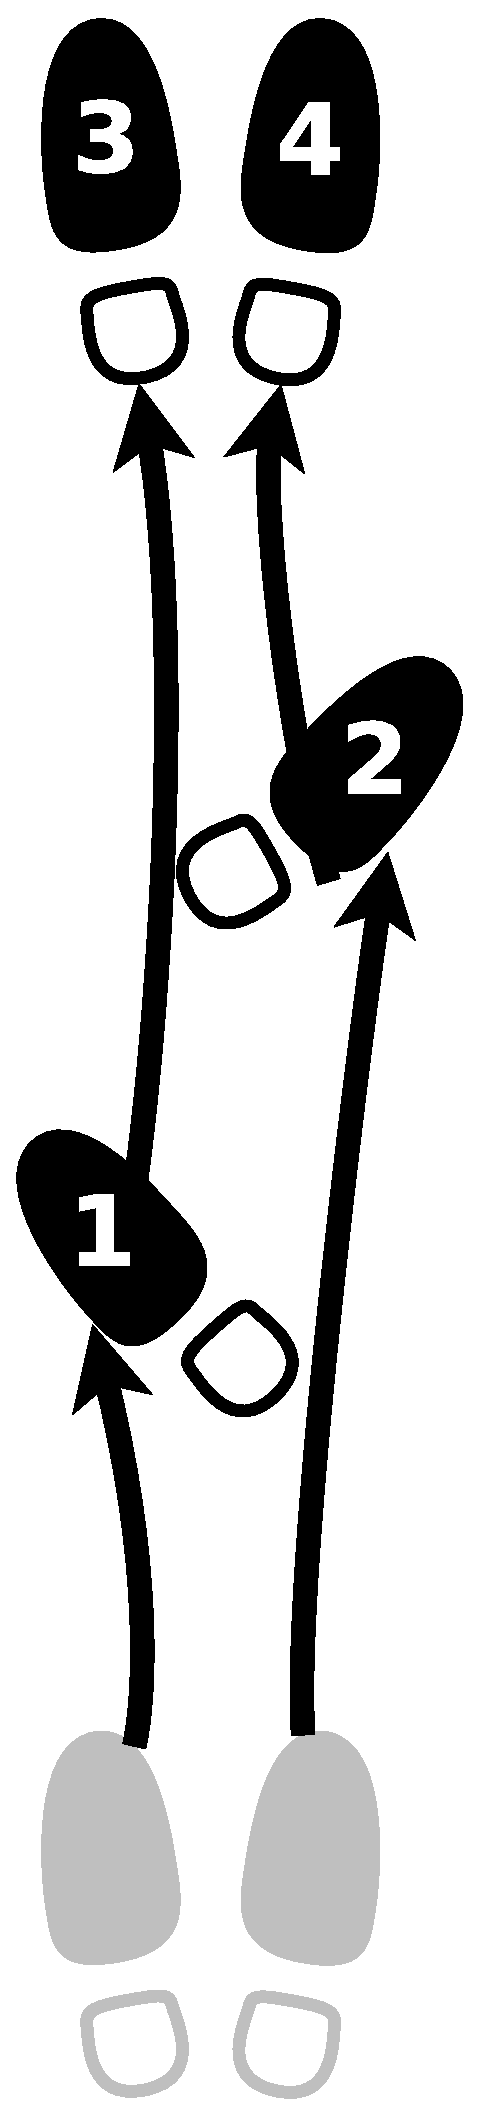
\includegraphics[width=0.3\textwidth]{chapters/cap-historia-dancasamba/samba-liso-basico-frente.eps}
        \caption{Passo básico para a frente.}
        \label{fig:samba-liso-basico-frente}
    \end{subfigure}
    ~ %add desired spacing between images, e. g. ~, \quad, \qquad, \hfill etc. 
      %(or a blank line to force the subfigure onto a new line)
    \begin{subfigure}[b]{0.3\textwidth}
        \centering
	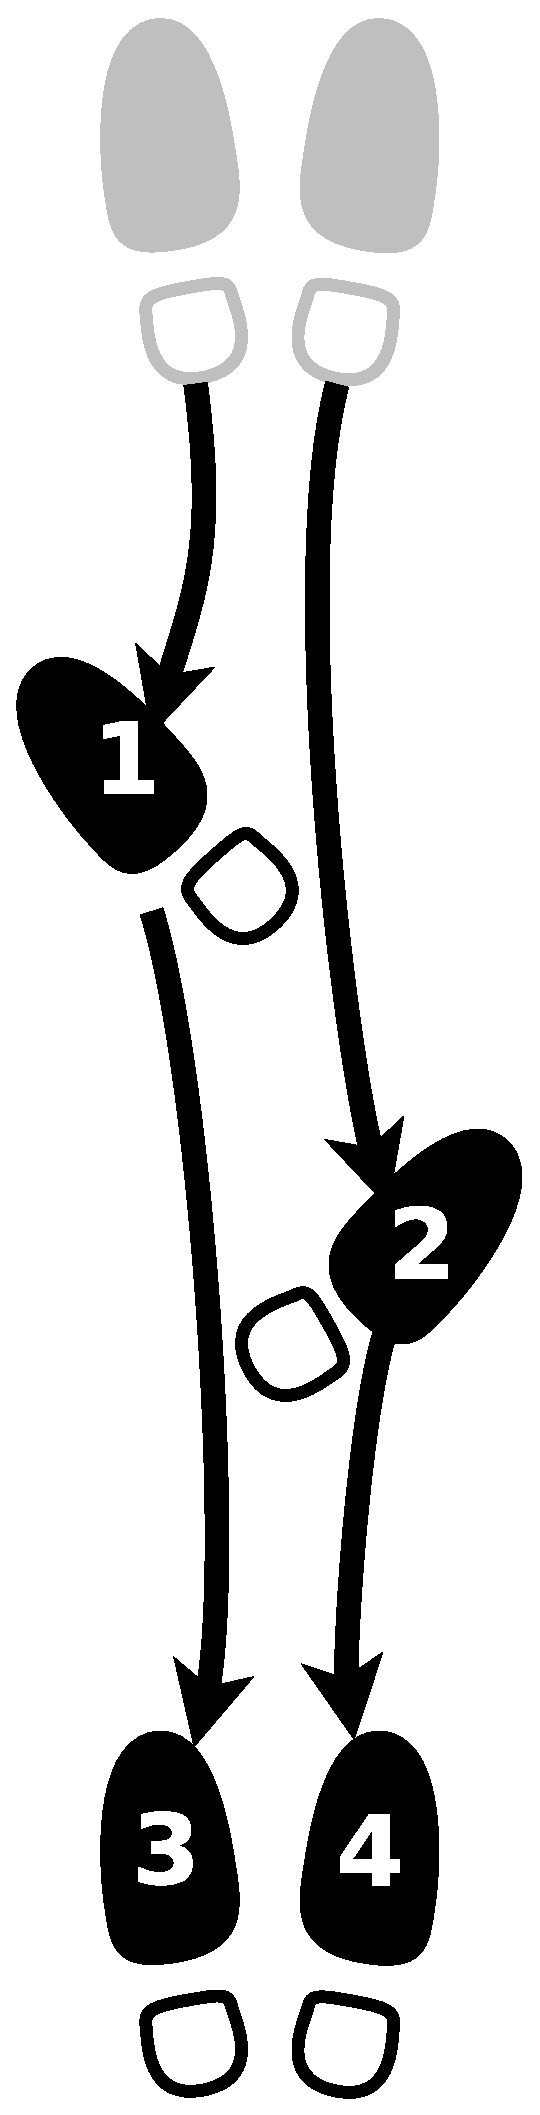
\includegraphics[width=0.3\textwidth]{chapters/cap-historia-dancasamba/samba-liso-basico-tras.eps}
        \caption{Passo básico para trás.}
        \label{fig:samba-liso-basico-tras}
    \end{subfigure}
    \caption{Samba liso da década de 1950.}\label{fig:samba-liso-basico}
\end{figure}

%%%%%%%%%%%%%%%%%%%%%%%%%%%%%%%%%%%%%%%%%%%%%%%%%%%%%%%%%%%%%%%%%%%%%%%%%%%%%%%%
\subsection{Samba pagode} 
\index{Dança!Samba pagode}
É um estilo de dança a dois, originário de São Paulo, 
é uma dança com poucos deslocamentos \cite[pp. 134]{perna2002samba}.
É um estilo de dança adaptado para ser dançado com o pagode paulista,
também chamado como Sambalanço\footnote{Ver página \pageref{ref:sambalanco}}.
%% https://www.youtube.com/watch?v=SfvoiXOGPn4
Ao igual que o sambalanço teve duas épocas com estilos musicais diferentes,
a dança \textbf{samba pagode}, sofreu também transformações acompanhando essas tendencias.
Podem-se observar atualmente 3 tipos de passo base: 
%% https://www.youtube.com/watch?v=rq1uhNXySds 
%% https://www.youtube.com/watch?v=SfvoiXOGPn4

O miudinho, que é um passo que se realiza abraçado com o par e de forma espelhada com este,
onde se executam 3 twist\footnote{É importante ter um sapato que deslise bem.} no lugar, 
só trocando de peso entre os pés, seguindo um ritmo, rápido-rápido-lento;
este movimento se executa simetricamente duas vesses para formar um ciclo completo,  
uma vez iniciando com o peso do corpo para o pé direito\footnote{Quando o primeiro twist é horário.} e a outra com o esquerdo.

O passo básico lateral, se realiza abraçado com o par  e de forma espelhada com este, 
é similar ao passo básico de capoeira,
ou a base aberta do forró\footnote{Só que aqui é abraçados.},
onde se produzem 3 movimento seguindo um ritmo, rápido-rápido-lento,
no primeiro momento, um pé vai para atrás, 
no segundo o outro ajeita sua posição deslocando-se levemente, 
procurando o centro e o equilíbrio do par dançante, e
no terceiro o pé que estava atrás volta ao lado do outro,
este movimento se executa simetricamente duas vesses para formar um ciclo completo,  
uma vez iniciando com pé direito e a outra com o esquerdo.
Este movimento é interessante para fazer deslocamento, 
que são realizados principalmente nesse primeiro movimento com o pé atrás, 
só que agora apontando para uma direção especifica.

A caidinha, se realiza abraçado com o par, 
este passo é similar ao picadilho (picadinho) de samba de gafieira,
porem com um deslocamento similar ao repique do forró;
no pagode paulista este movimento se executa seguindo um ritmo, rápido-rápido-lento,
onde o seguidor faz um movimento similar ao miudinho antes mencionado,
enquanto que o condutor tem uma liberdade criativa no 
seu movimento\footnote{O mesmo que acontece no picadilho de samba de gafieira.} 
enquanto respeite o ritmo, rápido-rápido-lento.

%%%%%%%%%%%%%%%%%%%%%%%%%%%%%%%%%%%%%%%%%%%%%%%%%%%%%%%%%%%%%%%%%%%%%%%%%%%%%%%%
\subsection{Samba rock (dança)}
\index{Dança!Samba rock}
É um estilo de dança a dois, realizado nos bailes ``black'' paulistas desde a década de 1960, 
sendo esta uma dança variante das danças do swing/rock e parente do soltinho carioca \cite[pp. 135]{perna2002samba}.
se dança bem em: Swing, samba rock (música), samba com suingue e samba-funk \cite[pp. 135,138]{perna2002samba}.
O samba rock se dança de mão dadas, e se carateriza por ter muitas voltas,
executadas na maior parte de vesses pelas  seguidores;
porem, é uma dança estacionaria pois os dançantes rara vez se deslocam pelo salão, 
e pelo contrario ficam trabalhando seus passos num mesmo lugar  \cite[pp. 135,138]{perna2002samba}.
Quando um espectador externo vê esta dança perceberá muitas figuras usando só os braços,
com enrosques, voltas, enlaces, etc.
Enquanto os pés de ambos dançarinos fazem uma mesma marcação, num constante e repetitivo rápido-rápido-lento,
caminhando unicamente sobre um circulo imaginário no chão, uma vez em sentido horário e outra em anti-horário.

%%%%%%%%%%%%%%%%%%%%%%%%%%%%%%%%%%%%%%%%%%%%%%%%%%%%%%%%%%%%%%%%%%%%%%%%%%%%%%%%
\subsection{Samba funkeado}
\index{Dança!Samba funkeado}
Também é chamado de estilo Jimmy de Oliveira ou simplesmente  samba Jimmy, 
em aluição a seu criador.
Este estilo de dança a dois foi criado no ano de 1998.
Com muito esforço Jimmy, num período aproximado de 6 meses, 
criou a estrutura da dança, desde iniciante ate avançado;
no ano de 1999 ele  chamou a esse estilo como ``samba quebrado'';  
posteriormente renomeou  para ``samba Jimmy'', 
recebeu algumas criticas e no ano 2001 decidiu renomeá-lo para ``samba funk'',
porem isto trouxe confusões   ao ser associado com a música funk, existente em Rio de Janeiro,
muito distante da proposta dele, e
finalmente a meados do 2005 ele decidiu chamá-lo ``samba funkeado''  \cite{sambafunkeadoJimmyDeOliveiraPart1}.
A Figura \ref{fig:funkeadocrono1} mostra a cronologia de nomes para este estilo.
\begin{figure}[h]
  \centering
    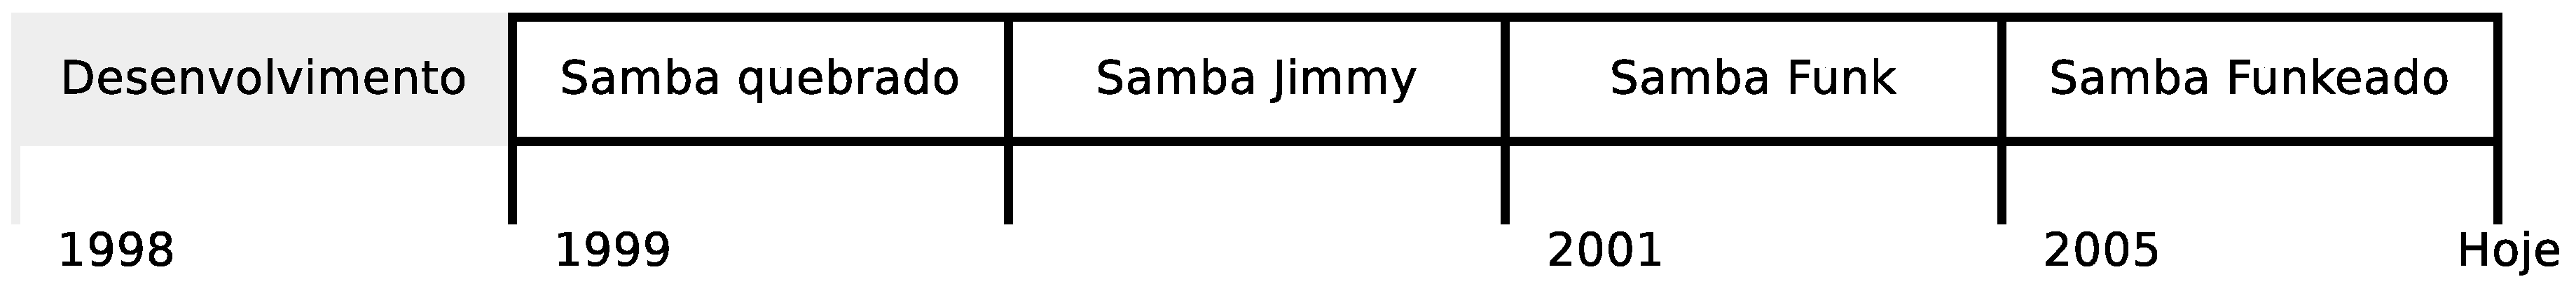
\includegraphics[width=0.85\textwidth]{chapters/cap-historia-dancasamba/sambafunkeado.eps}
  \caption{Cronologia dos nomes para samba funkeado.}
\label{fig:funkeadocrono1}
\end{figure}

O estilo foi criado para, em palavras de Jimmy: ``contribuir em função da música'', 
numa tentativa de agregar movimento em coerência como as músicas que ele gostava;
sendo estas interpretadas por:
Djavan, Jorge Ben Jor, Tim Maia, Leny Andrade \cite{sambafunkeadoJimmyDeOliveiraPart1}, que em seu momento, 
presentaram músicas de bossa nova ou que eram influenciadas pelo jazz, 
funk norte-americano ou ``black music'' \cite{sambafunkeadoJimmyDeOliveiraPart1} \cite{sambafunkeadoJimmyDeOliveiraPart3},
Jimmy indica que seu estilo procura ir em função da música escutada no brasil, 
e que a maioria da música atual é influenciada pelo funk norte-americano;
como a música de: João Sabiá. 

O samba funkeado pode ser dançado em gêneros como ``black music'',
em pagodes funkeados (Sorriso maroto, Netinho de Paula, pixote, etc.), 
em sambas com influencia do jazz \cite{sambafunkeadoJimmyDeOliveiraPart3}, etc. 

O samba funkeado tem 3 tendencias ou estruturas  \cite{sambafunkeadoJimmyDeOliveiraPart2}:
\begin{itemize}
\item \textbf{Samba funkeado}, primigênio.
\item \textbf{Samba funkeado fragmentado}; exemplo: um movimento que é de sentar, que gastaria um tempo, 
passa a ter ate 3 tempos; é dizer, fragmenta os movimentos. 
O fragmentado também permite dançar com movimentações em contrapeso no par de dança.
\item \textbf{Samba funkeado samsurf}, com uma postura mais curvada.
\end{itemize}

%e em seu ídolo Michael Jackson \cite{sambafunkeadoJimmyDeOliveira2}.
 
%%%%%%%%%%%%%%%%%%%%%%%%%%%%%%%%%%%%%%%%%%%%%%%%%%%%%%%%%%%%%%%%%%%%%%%%%%%%%%%%
\subsection{Samba internacional} 
\index{Dança!Samba internacional}
É um estilo de dança a dois, influenciado pelo maxixe;
se dança principalmente fora do Brasil e existem basicamente dois estilos: 
o estilo internacional e o estilo norte-americano (EE.UU.) \cite[pp. 134-135]{perna2002samba}.

O samba introduzida a EE.UU. é uma dança de salão muito animada, 
com música de ritmo alegre, que sugere um estilo de movimento que pode
chegar a ser tão turbulento quanto os movimentos do Jive.
O padrão de passos básicos é similar aos achados no Fox-Trot e o Waltz,
sendo estes: fwd-swd-close ... bwd-swd-close; e
tem passos com tempos que seguem uma sequência: 
quick-quick-slow\footnote{Rápido-rápido-lento.} ... quick-quick-slow \cite{parson2016ballroom}.

Observando os campeonatos internacionais onde este estilo é usado, 
se percebe que o samba internacional é dançado em qualquer estilo musical que
tenha sotaque ou de a impressão de ter raiz afro-latina.

%%%%%%%%%%%%%%%%%%%%%%%%%%%%%%%%%%%%%%%%%%%%%%%%%%%%%%%%%%%%%%%%%%%%%%%%%%%%%%%%
\subsection{Relações entre os subgêneros do samba e os estilos de dançados em pares}

A Figura \ref{fig:sambadavavsmusica} mostra as relações entre os estilos de dança a dois (na esquerda),
 e os subgêneros do samba (na direita) \cite[pp. 134-138]{perna2002samba}.

\begin{figure}[h]
  \centering
    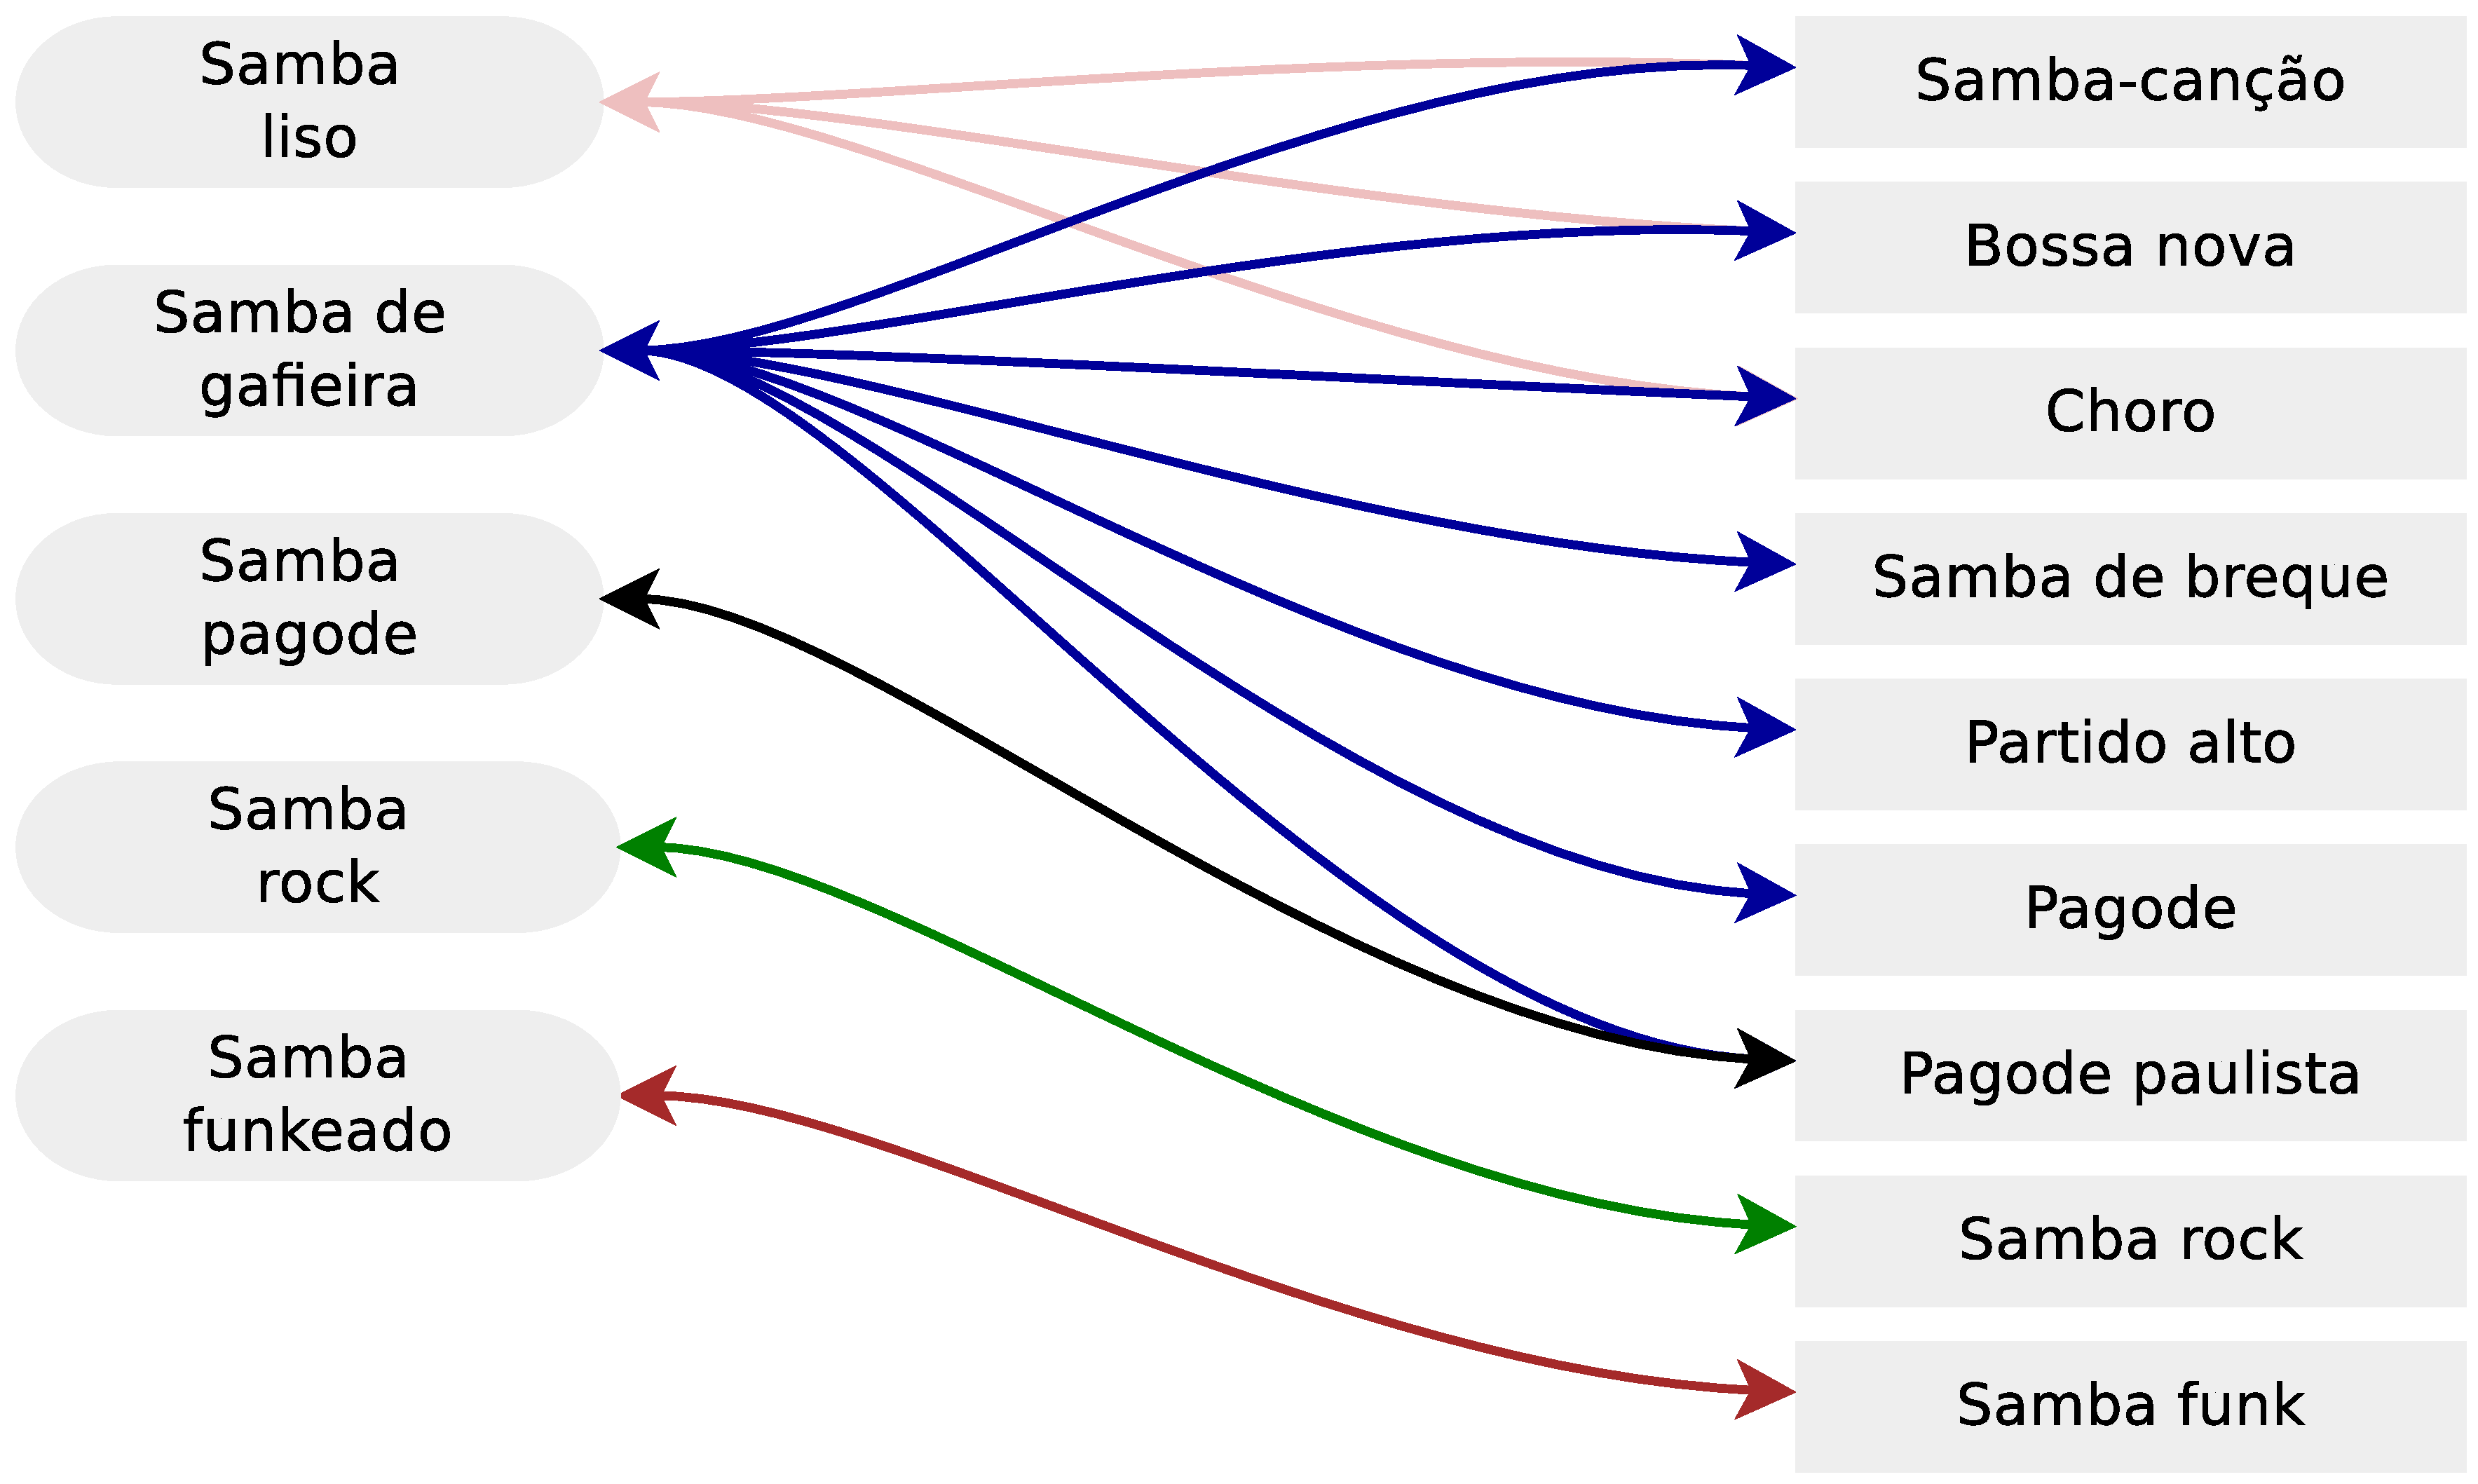
\includegraphics[width=0.8\textwidth]{chapters/cap-historia-dancasamba/dancavcmusica.eps}
  \caption{Relações entre os estilos de dança a dois e os subgêneros do samba.}
\label{fig:sambadavavsmusica}
\end{figure}

%%%%%%%%%%%%%%%%%%%%%%%%%%%%%%%%%%%%%%%%%%%%%%%%%%%%%%%%%%%%%%%%%%%%%%%%%%%%%%%%
%%%%%%%%%%%%%%%%%%%%%%%%%%%%%%%%%%%%%%%%%%%%%%%%%%%%%%%%%%%%%%%%%%%%%%%%%%%%%%%%
\section{Estilos dançados de forma separada}
Entre os estilos que se dançam de forma separada temos \cite[pp. 134]{perna2002samba}:

\subsection{Samba reggae  (dança)} 
Este estilo de samba que se dança separado, 
é uma dança baiana também conhecida como axé-dance, samba baiano ou pagode baiano,
se dança em samba reggae (música) \cite[pp. 134]{perna2002samba}.

\subsection{Samba no pé} 
É o estilo usado nas quadras das escolas de samba,
se dança bem em estilos musicais como: 
samba enredo ou em qualquer samba rápido  \cite[pp. 134]{perna2002samba}.

\subsection{Marcha de carnaval}
 É uma dança própria do carnaval para se dançar em cordões.
se dança bem em: marchas, marchas-rancho e samba-enredo lentos  \cite[pp. 135]{perna2002samba}.


\subsection{Relações entre os subgêneros do samba e os estilos de dançados separadamente}

A Figura \ref{fig:sambadavavsmusicaseparado} mostra as relações existentes, 
entre os estilos de dança que se dançam separados (na esquerda) 
e alguns subgêneros do samba (na direita)  \cite[pp. 134-138]{perna2002samba}.

\begin{figure}[h]
  \centering
    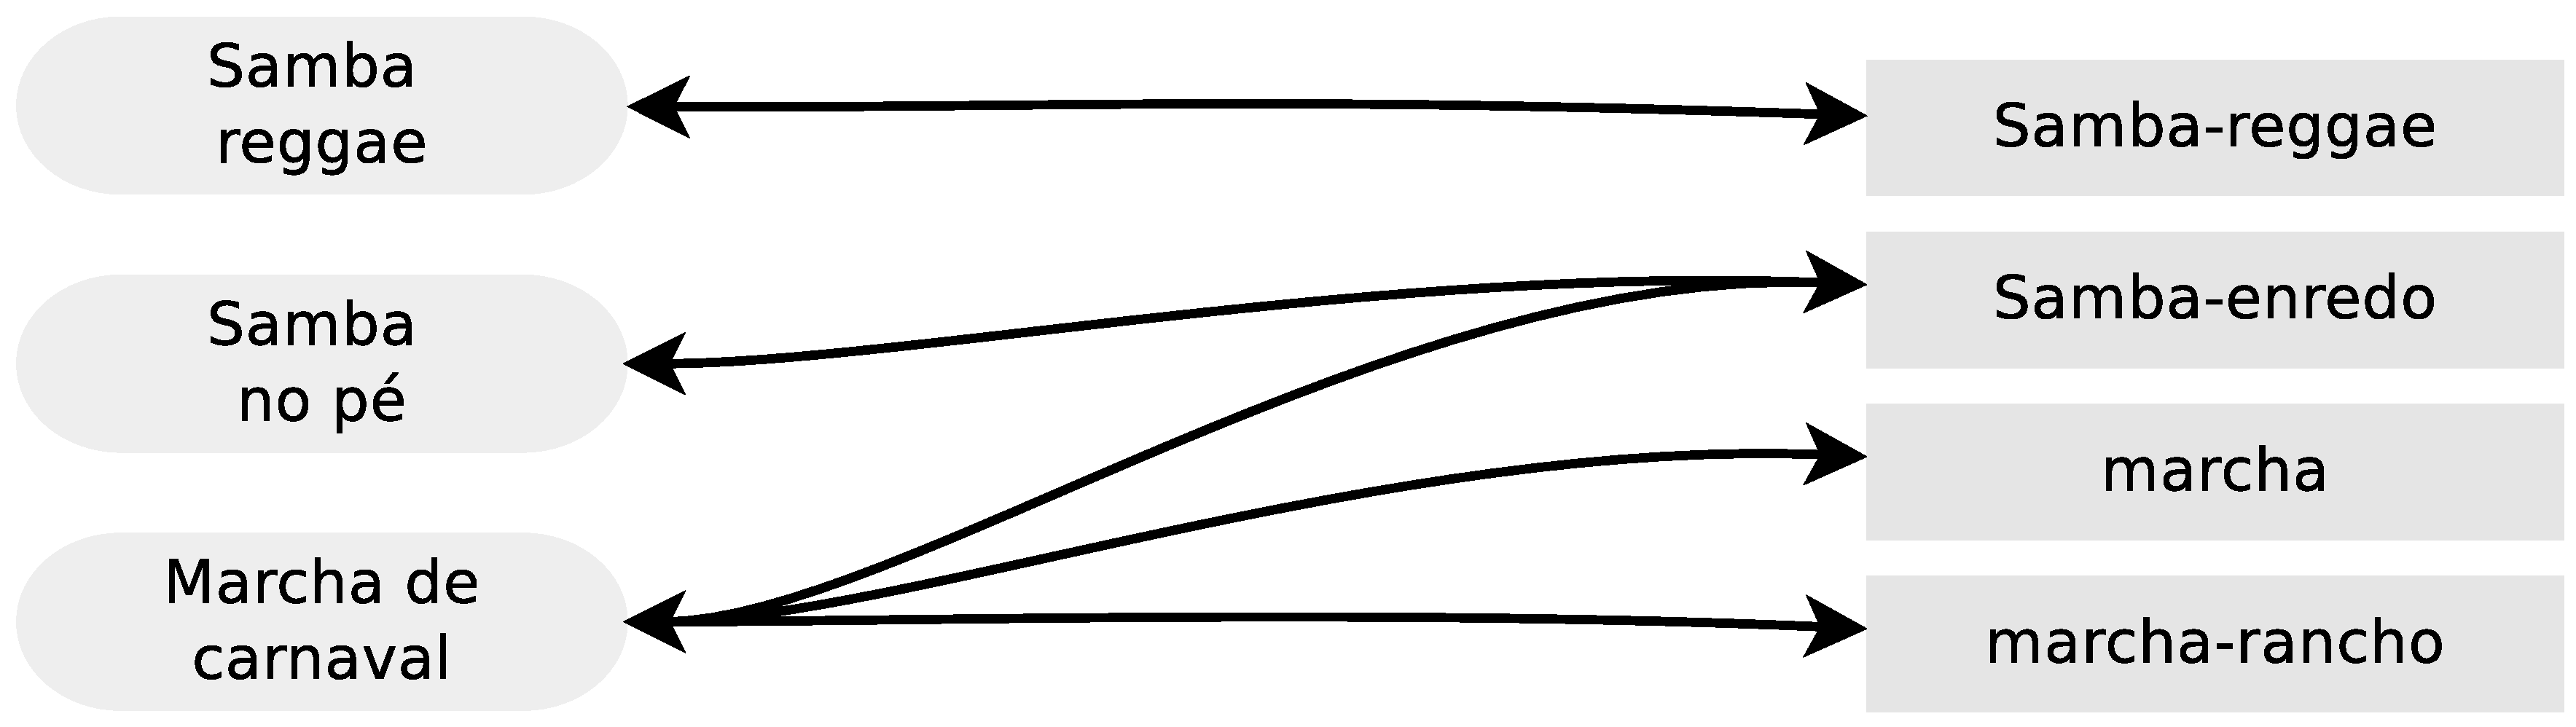
\includegraphics[width=0.6\textwidth]{chapters/cap-historia-dancasamba/dancavcmusicaseparado.eps}
  \caption{Relações entre os estilos de dança (separados) e os subgêneros do samba.}
\label{fig:sambadavavsmusicaseparado}
\end{figure}
